
\section{Slowing Down, Speeding Up, and Turning\footnote{
1990-93 Dept. of Physics and Astronomy, Dickinson College. Supported by FIPSE
(U.S. Dept. of Ed.) and NSF. Portions of this material may have been modified
locally and may not have been classroom tested at Dickinson College.
}}

\makelabheader %(Space for student name, etc., defined in master.tex or labmanual_formatting_commands.tex)

\medskip
\textbf{Objectives }

\begin{itemize}
\item To learn how to relate graphs of acceleration \textit{vs.}~time to the motions they represent. 
\item To understand the relationship between velocity \textit{vs.}~time and acceleration vs.
time graphs.
\end{itemize}

\medskip
\textbf{About Slowing Down, Speeding Up and Turning }

In the previous session, you explored the characteristics of position \textit{vs.}~time,
velocity \textit{vs.}~time and acceleration  \textit{vs.}~time graphs of the motion of a dynamics
cart. In the cases examined, the cart was always moving away from a motion detector,
either at a constant velocity or with a constant acceleration. Under these conditions,
the velocity and acceleration are both positive. You also learned how to find
the magnitude of the acceleration from velocity \textit{vs.}~time and acceleration vs.
time graphs, and how to represent the velocity and acceleration using vectors. 

In the motions you studied in the last session, the velocity and acceleration
vectors representing the motion of the cart both pointed in the same direction.
In order to get a better feeling for acceleration, it will be helpful to examine
velocity \textit{vs.}~time and acceleration \textit{vs.}~time graphs for some slightly more complicated
motions of a cart on an inclined track. Again you will use the motion detector
to observe the cart as it changes its velocity at a constant rate. Only this
time the motion may be toward the detector, and the cart may be speeding up
or slowing down.

\medskip
\textbf{Apparatus }

\begin{itemize}
\item \textit{Science Workshop 750 Interface}
\item Ultrasonic motion detector 
\item \textit{DataStudio} software (P, V \& A Graphs application)
\item Collision cart and track 
\item Lab stand to incline the track
\end{itemize}

\medskip
\textbf{Slowing Down and Speeding Up }

In this activity you will look at a cart moving along an inclined track and
slowing down. A car being brought to rest by the steady action of brakes is
a good example of this type of motion. Later you will examine the motion of
the cart toward the motion detector and speeding up. In both cases, we are interested
in the shapes of the velocity \textit{vs.}~time and acceleration \textit{vs.}~time graphs, as
well as the vectors representing velocity and acceleration. 

Let's start with the creation of velocity and acceleration graphs of when it
is moving away from the motion detector and slowing down. To do this activity,
the track should be inclined with a lab stand at one end and the motion detector set up at the lower end of the track. Adjust the lab stand so that the track is raised a few centimeters at the opposite end from where the motion detector is located. Now when you give the cart a push away from the motion detector, it will slow down after it is released. In this activity you will examine the velocity and acceleration of this motion.

\pagebreak[2]
\textbf{Activity 1: Graphs Depicting Slowing Down} 

(a) If you give the cart a push away from the motion detector and release it,
will the acceleration be positive, negative or zero (after it is released)?
Sketch your predictions for the velocity \textit{vs.}~time and acceleration \textit{vs.}~time
graphs on the axes below using dashed lines.

\vspace{0.3cm}
{\par\centering 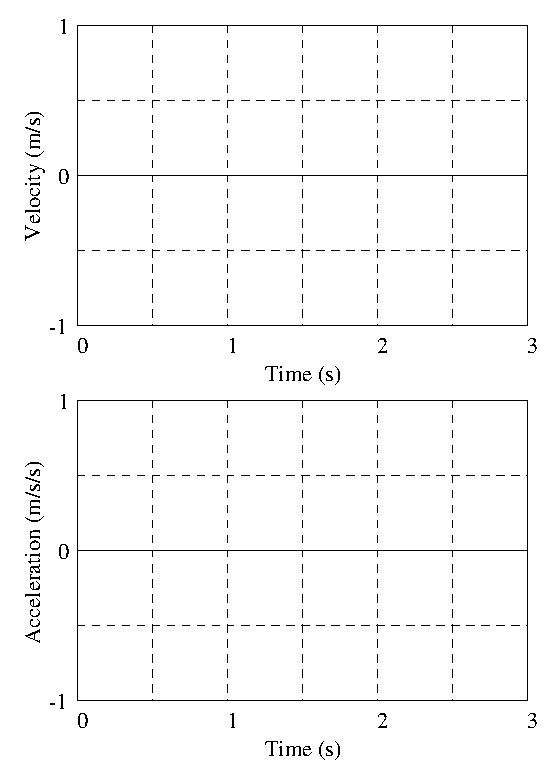
\includegraphics{slowing/slowing_fig1.eps} \par}
\vspace{0.3cm}

(b) To test your predictions, open the \textbf{P, V \& A Graphs} application as you did in the previous experiment. Locate the cart 0.15 m from the motion detector and gently push the cart away from the motion detector once it starts clicking. Catch the cart \underline{before} it turns around or hits the end of the track.

Draw the results on the axes above using solid lines for the part of the motion
after the cart is released. You may have to try a few times to get a good run.  The acceleration \textit{vs.}~time graphs will exhibit small fluctuations due to irregularities in the motion of the cart. You should ignore these fluctuations and draw smooth patterns.

(c) Did the shapes of your velocity and acceleration graphs agree with your
predictions? How is the sign of the acceleration represented on a velocity vs.
time graph? 
\answerspace{15mm}

(d) How is the sign of the acceleration represented on an acceleration \textit{vs.}~time
graph? 
\answerspace{15mm}

\pagebreak[3]
(e) Is the sign of the acceleration what you predicted? How does slowing down
while moving away from the detector result in this sign of acceleration? Hint:
Remember that acceleration is the rate of change of velocity. Look at how the
velocity is changing.
\answerspace{20mm}

%\textbf{Constructing Acceleration Vectors for Slowing Down }
\textbf{Activity 2: Constructing Acceleration Vectors for Slowing Down}

Let's consider a diagrammatic representation of a cart which is slowing down
and use vector techniques to figure out the direction of the acceleration.

%\textbf{Activity 2: Vector Diagrams for Slowing Down} 

(a) The diagram that follows shows the positions of the cart at equal time intervals.
(This is like taking snapshots of the cart at equal time intervals.) At each
indicated time, sketch a vector above the cart which might represent the velocity
of the cart at that time while it is moving away from the motion detector and
slowing down.

\vspace{0.5cm}
%{\par\centering 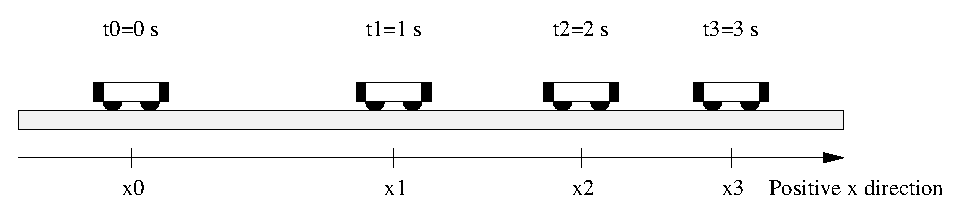
\includegraphics{slowing/slowing_fig2.eps} \par}
{\par\centering 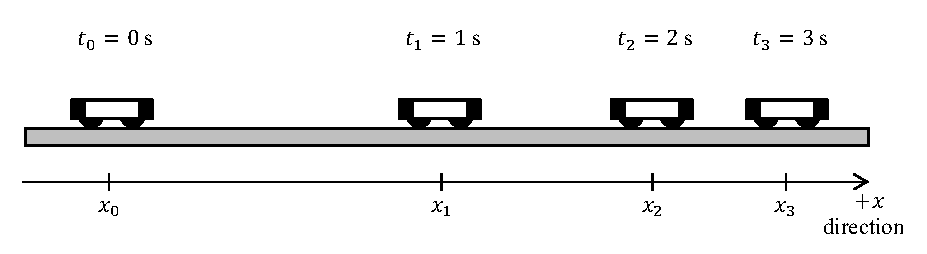
\includegraphics{slowing/carts_slowing.eps} \par}
\vspace{0.5cm}

(b) Show below how you would find the vector representing the change in velocity
between the times 1s and 2s by creating a vector diagram using the vectors 
 above. Based on the direction of the resultant vector and the direction of 
the positive x-axis, what is the sign of the acceleration? 
Does this agree with your answer to Question (e) in Activity 1?
\answerspace{25mm}

(c) By filling in the following table, state the general rules to predict the 
sign of the acceleration if you know the sign of the velocity (i.e., the 
direction of motion) and whether the object is speeding up or slowing down. 
Positive velocities have been investigated in this experiment and the previous 
one. Negative velocities we investigate below, so these are essentially 
predictions.

\vspace{0.3cm}
{\centering \begin{tabular}{|c|c|c|}
\hline
Velocity&
&
Acceleration\\
\hline
positive&
speeding up&
\\
\hline
positive&
slowing down&
\\
\hline
negative&
speeding up&
\\
\hline
negative&
slowing down&
\\
\hline
\end{tabular}\par}
\vspace{0.3cm}


%\newpage
\pagebreak[2]
\textbf{Activity 3: Speeding Up Toward the Motion Detector} 

Suppose the cart is allowed to speed up when traveling toward the motion 
detector. What will be the sign of the acceleration? Positive or negative? 

(a) Use the general rules that you stated in Activity 2 to predict the shapes
of the velocity and acceleration graphs. Sketch your predictions using dashed
lines on the axes that follow.

%\vspace{0.3cm}
{\par\centering 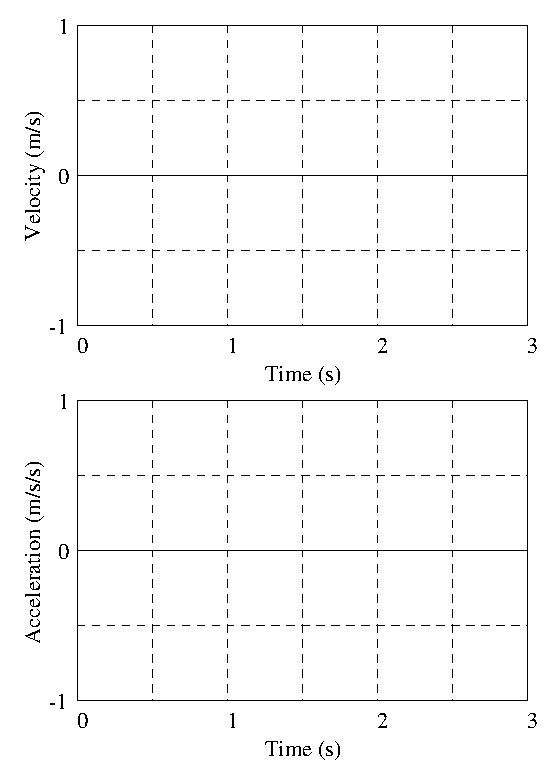
\includegraphics{slowing/slowing_fig1.eps} \par}
%\vspace{0.3cm}

(b) Test your predictions by releasing the cart from rest at the raised end of the track after the motion detector starts clicking. Catch the cart before it gets too close to the detector.  
Draw the results using solid lines on the axes above. You may have to try a
few times to get a good run.

(c) How does your velocity graph show that the cart was moving toward the detector? 
\answerspace{20mm}

(d) During the time that the cart was speeding up, is the acceleration positive
or negative? Does this agree with your prediction? Explain how speeding up while
moving toward the detector results in this sign of acceleration. Hint: Think
about how the velocity is changing.
\answerspace{20mm}

\pagebreak[2]
\textbf{Activity 4: Constructing Acceleration Vectors for Speeding Up} 

Let's consider a diagrammatic representation of a cart which is speeding up
and use vector techniques to figure out the direction of the acceleration.

(a) The diagram that follows shows the positions of the cart at equal time intervals.
(This is like taking snapshots of the cart at equal time intervals.) At each
indicated time, sketch a vector above the cart which might represent the velocity
of the cart at that time while it is moving toward the motion detector and speeding
up.

%\vspace{0.3cm}
%{\par\centering 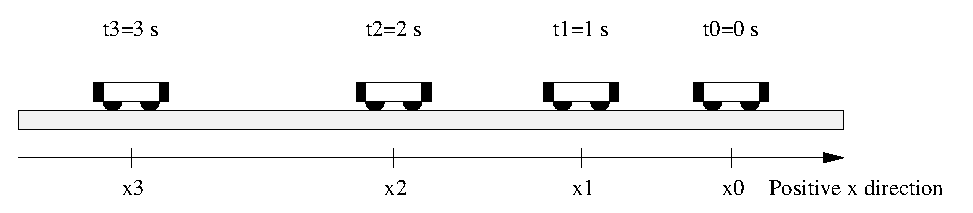
\includegraphics{slowing/slowing_fig3.eps} \par}
{\par\centering 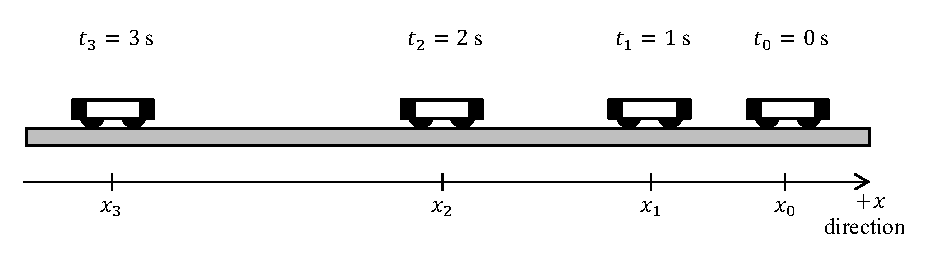
\includegraphics{slowing/carts_speeding.eps} \par}
%\vspace{0.3cm}

(b) Show below how you would find the vector representing the change in velocity
between the times 1s and 2s as you did in Activity 2(b). Based on the 
direction of the resultant vector and the direction of the positive x-axis, 
what is the sign of the acceleration? 
Does this agree with your answer to Question (d) in Activity 3?
\vspace{20mm}

\textbf{Activity 5: Moving Toward the Detector and Slowing Down }

There is one more possible combination of velocity and acceleration for the
cart, that of moving toward the detector while slowing down. 

%Slowing Down Toward the Detector} 

(a) Use your general rules to predict the direction and sign of the acceleration
when the cart is slowing down as it moves toward the detector. Explain why the
acceleration should have this sign in terms of the velocity and how the 
velocity is changing. 
\answerspace{15mm}

(b) The diagram below shows the positions of the cart at equal time intervals
for slowing down while moving toward the detector. At each indicated time, 
sketch
a vector above the cart which might represent the velocity of the cart at that
time while it is moving toward the motion detector and slowing down.

%\vspace{0.3cm}
%{\par\centering 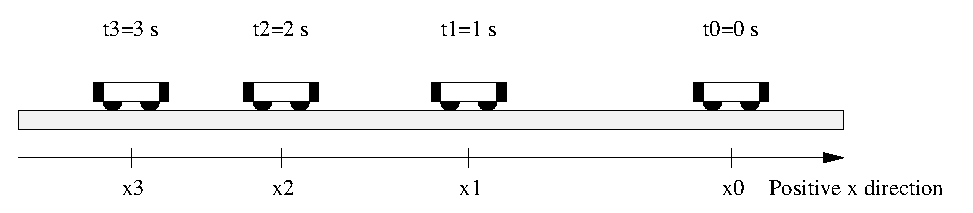
\includegraphics{slowing/slowing_fig4.eps} \par}
{\par\centering 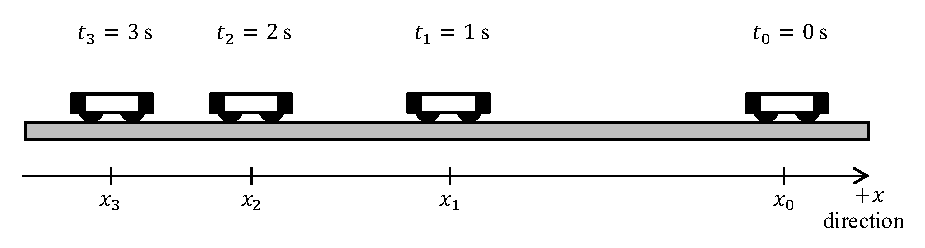
\includegraphics{slowing/carts_slowing2.eps} \par}
%\vspace{0.3cm}

(c) Show below how you would find the vector representing the change in velocity
between the times 1~s and 2~s as you did in Activity 2(b). Based on the 
direction of the resultant vector and the direction of the positive $x$ axis, 
what is the sign of the acceleration? 
Does this agree with the prediction you made in part (a)?
\answerspace{10mm}

\pagebreak[2]
\textbf{Activity 6: Acceleration and Turning Around }

In Lab \ref{changing_motion}, and in Activity 1 in this session, you looked at
velocity \textit{vs.}~time and acceleration \textit{vs.}~time graphs for a cart moving in one
direction with a changing velocity. In this investigation you will look at what
happens when the cart slows down, turns around and then speeds up. (This is a
combination of Activities 1 and 3.)

To practice this motion you should position the cart 0.15 m from the detector
and give the cart a gentle push away from the motion detector. It should move
up the track, slow down, reverse direction and then move back down toward the
detector. Try it without activating the motion detector! Be sure that the cart
does not hit the end of the track before it turns around. 

%\textbf{Activity 6: Reversing Direction }

(a) For each part of the motion-away from the detector, at the turning point,
and toward the detector, predict in the table that follows whether the velocity
will be positive, zero or negative. Also indicate whether the acceleration is
positive, zero or negative.

\vspace{0.3cm}
{\centering \begin{tabular}{|c|c|c|c|}
\hline 
&
Moving Away&
Turning Around&
Moving Toward\\
\hline 
Velocity&
&
&
\\
\hline 
Acceleration&
&
&
\\
\hline 
\end{tabular}\par}
\vspace{0.3cm}

(b) Sketch the predicted shapes of the velocity \textit{vs.}~time and acceleration 
\textit{vs.}~time graphs of this entire motion on the axes that follow using dashed lines.

\vspace{0.3cm}
{\par\centering 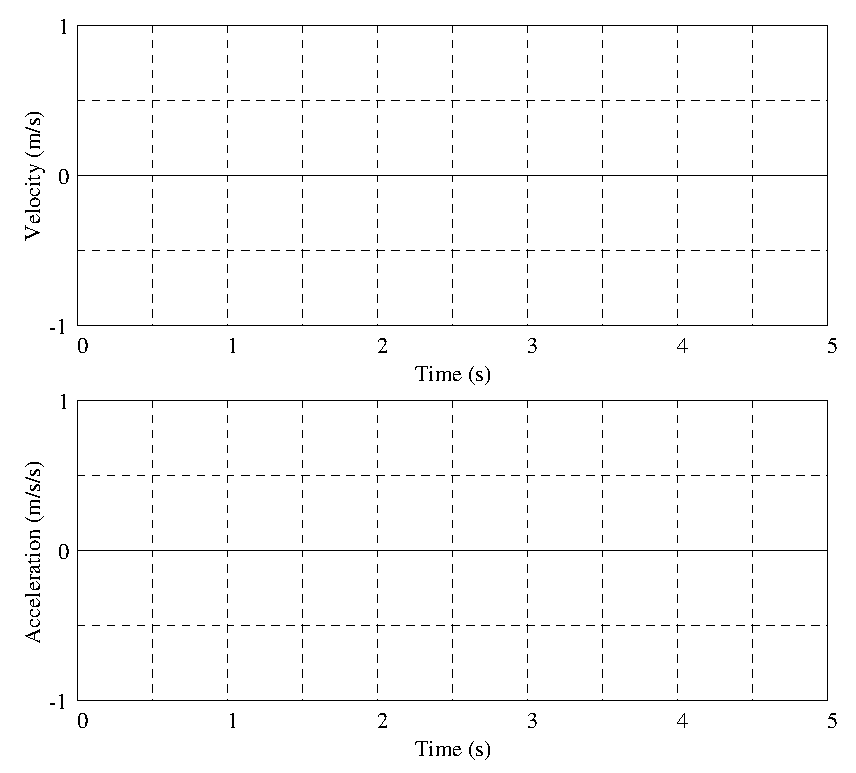
\includegraphics{slowing/slowing_fig5.eps} \par}
%\vspace{13mm}

(c) Test your predictions by making graphs of the motion. Use the procedures
you used in the slowing down and speeding up activities. You may have to try
a few times to get a good run. When you get a good run, sketch both graphs on the axes above using solid lines.

\pagebreak[2]
(d) Did the cart have a zero velocity at any point in the motion? (Hint: Look
at the velocity graph. What was the velocity of the cart at the end of the ramp?)
Does this agree with your prediction? How much time did it spend at zero velocity
before it started back toward the detector?
\answerspace{20mm}

(e) According to your acceleration graph, what is the acceleration at the instant
the cart comes to rest? Is it positive, negative or zero? Does this agree with
your prediction? 
\answerspace{20mm}

(f) Explain the observed sign of the acceleration at the end of the ramp. (Hint: Remember that acceleration is the rate of change of velocity.) 
\answerspace{20mm}

(g) If your instructor requests it, print a copy of the position, velocity, and acceleration graphs for each person in your group and add the graphs to this unit.

(h) Notice that the slope of the velocity graph is not quite the same for positive velocities as it is for negative velocities. (This difference can also be seen on the acceleration graph.) What accounts for this difference?
\answerspace{20mm}

%\textbf{Tossing a Ball }
\textbf{Activity 7: The Rise and Fall of a Ball} 

Suppose you throw a ball up into the air. It moves upward, reaches its highest
point and then moves back down toward your hand. We will now consider what can be said about the directions of its velocity and acceleration vectors at various points.

(a) Consider the ball toss carefully. Assume that upward is the positive direction.
Indicate in the table that follows whether the velocity is positive, zero or
negative during each of the three parts of the motion. Also indicate if the
acceleration is positive, zero or negative. Hint: Remember, to find the acceleration
you must look at the change in velocity.

\vspace{0.3cm}
{\centering \begin{tabular}{|c|c|c|c|}
\hline 
&
Moving Up&
At Highest Point&
Moving Down\\
&
(After Release)&
&
\\
\hline 
Velocity&
&
&
\\
\hline 
Acceleration&
&
&
\\
\hline 
\end{tabular}\par}
\vspace{0.3cm}

(b) In what ways is the motion of the ball similar to the motion of the cart
which you just observed?
\answerspace{10mm}

\pagebreak[3]
\textbf{Homework} 

1. An object moving along a line (the + position axis) has the acceleration-time graph below. How might the object move to create this graph if it is moving
\underline{toward the origin}?

\vspace{0.3cm}
{\par\centering 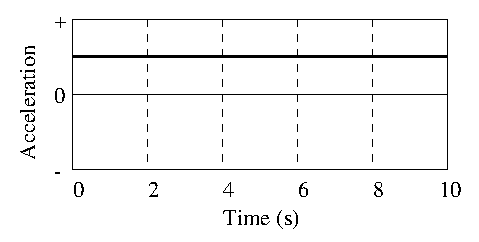
\includegraphics{slowing/slowing_fig6.eps} \par}
\vspace{0.3cm}

2. Sketch on the axes below the velocity-time graph that goes with the above
acceleration- time graph.

\vspace{0.3cm}
{\par\centering 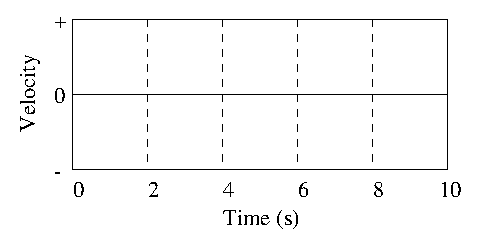
\includegraphics{slowing/slowing_fig7.eps} \par}
\vspace{0.3cm}

3. How would an object move to create each of the three labeled parts of the
acceleration-time graph shown below? (Consider the labeled straight line segments only, not the connectors between them.)

\vspace{0.3cm}
{\par\centering 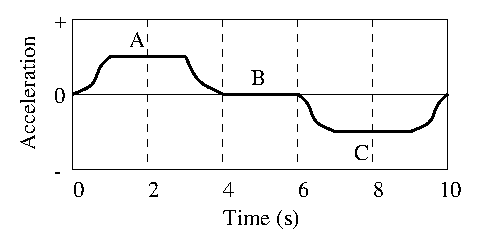
\includegraphics{slowing/slowing_fig8.eps} \par}
\vspace{0.3cm}

\hspace{20mm}A: 
\answerspace{10mm}

\hspace{20mm}B: 
\answerspace{10mm}

\hspace{20mm}C:
\answerspace{10mm}

\pagebreak[2]
4. Sketch below a velocity-time graph which might go with the acceleration-time
graph in question (3). (Again, consider the straight line segments only.)

\vspace{0.3cm}
{\par\centering 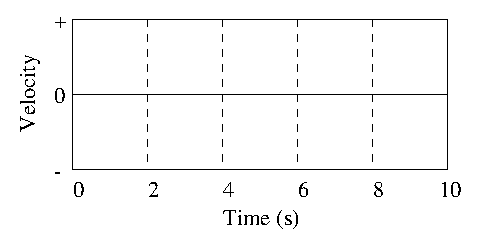
\includegraphics{slowing/slowing_fig9.eps} \par}
\vspace{0.3cm}

5. Sketch the shape of the acceleration-time graph that goes with the velocity-time
graph shown below.

\vspace{0.3cm}
{\par\centering 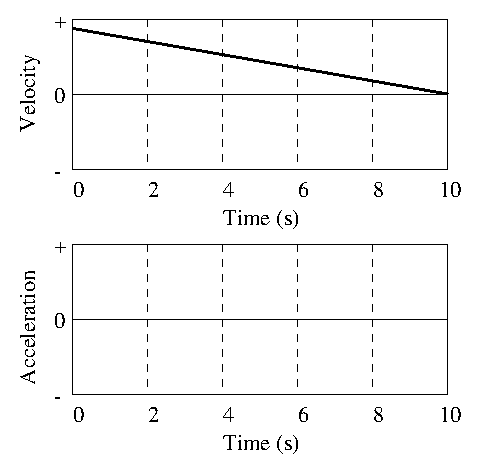
\includegraphics{slowing/slowing_fig10.eps} \par}
\vspace{0.3cm}

6. A car moves along a line {[}the + position axis{]}. Fill in the table below
with the sign (+ or -) of the velocity and acceleration of the car for each
of the motions described.

\vspace{0.3cm}
{\centering \begin{tabular}{|c|c|c|c|c|}
\hline 
&
Position&
Velocity&
Acceleration&
Acceleration\\
&
&
&
Speeding Up&
Slowing Down\\
\hline 
Car Moves Away&
+&
&
&
\\
from the Origin&
&
&
&
\\
\hline 
Car Moves Toward&
+&
&
&
\\
the Origin&
&
&
&
\\
\hline 
\end{tabular}\par}
\vspace{0.3cm}

\newpage

7. For each of the position-time graphs shown, sketch below it the corresponding
velocity- time and acceleration-time graphs.

%\vspace{0.3cm}
{\par\centering 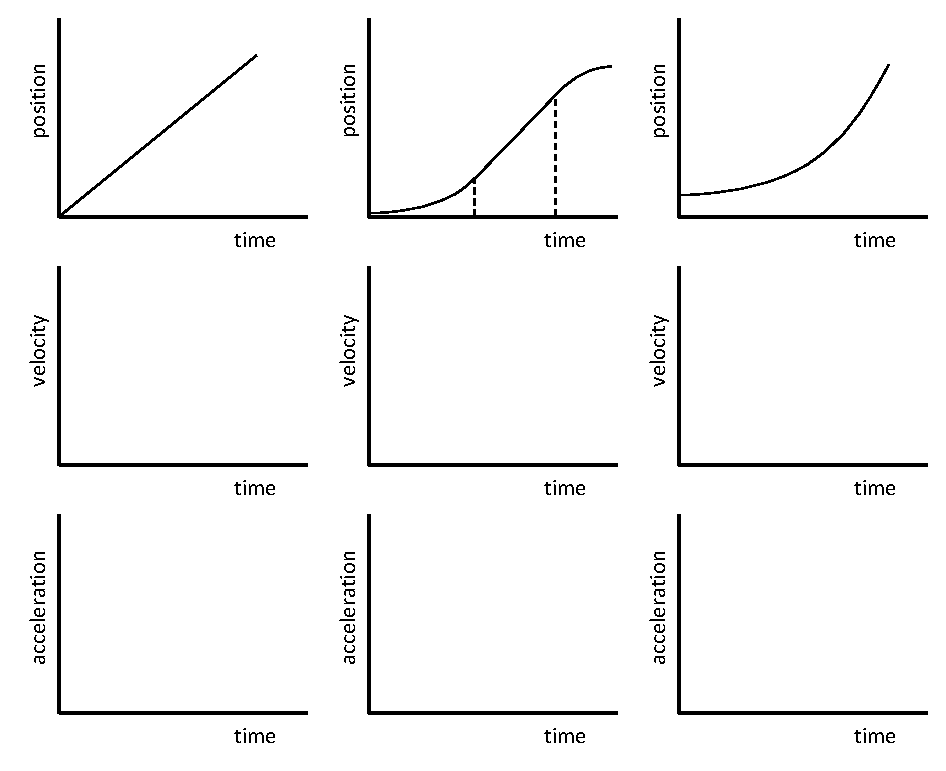
\includegraphics[width=0.85\textwidth]{slowing/slowing_fig11_new.eps} \par}
%\vspace{0.3cm}

8. Describe how you would move to produce the velocity-time graph shown below.

\vspace{0.3cm}
{\par\raggedright 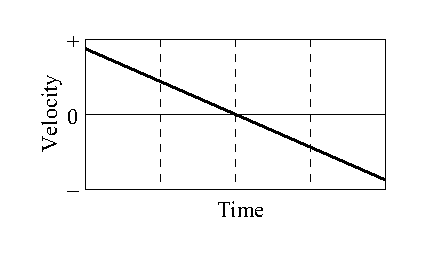
\includegraphics{slowing/slowing_fig12.eps} \par}
\vspace{0.3cm}

9. Sketch a position-time graph corresponding to the velocity-time graph above.

\vspace{0.3cm}
{\par\centering 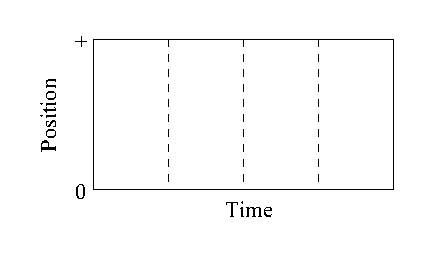
\includegraphics{slowing/slowing_fig13.eps} \par}
\vspace{0.3cm}

10. Sketch an acceleration-time graph corresponding to the velocity-time graph
above.

\vspace{0.3cm}
{\par\centering 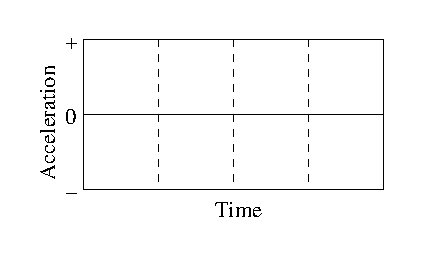
\includegraphics{slowing/slowing_fig14.eps} \par}
\vspace{0.3cm}

A car can move in either direction along a line (the + position axis). Sketch
velocity-time and acceleration-time graphs that correspond to each of the following
descriptions of the car's motion.

11. The car is moving toward the origin at a constant velocity.

\vspace{0.3cm}
{\par\centering 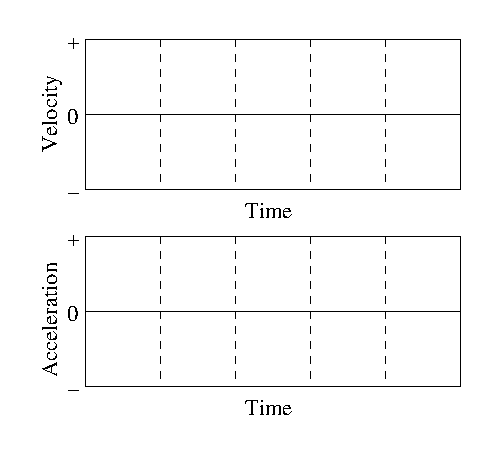
\includegraphics{slowing/slowing_fig15.eps} \par}
\vspace{0.3cm}

12. The car starts from rest and moves toward the origin, speeding up at a steady
rate.

\vspace{0.3cm}
{\par\centering 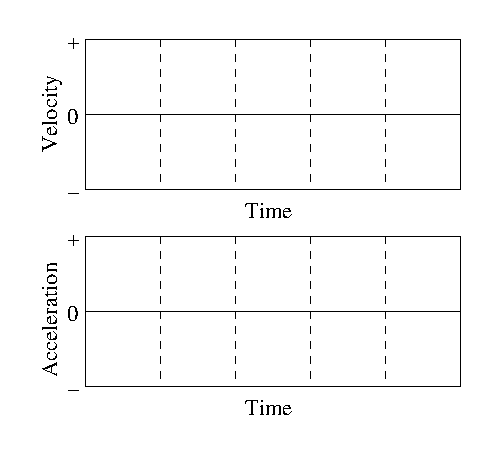
\includegraphics{slowing/slowing_fig15.eps} \par}
\vspace{0.3cm}

13. A ball is tossed in the air. It moves upward, reaches its highest point
and falls back downward. Sketch a velocity-time and an acceleration-time graph
for the ball from the moment it leaves the thrower's hand until the moment just
before it reaches her hand again. Consider the positive direction to be upward.

\vspace{0.3cm}
{\par\centering 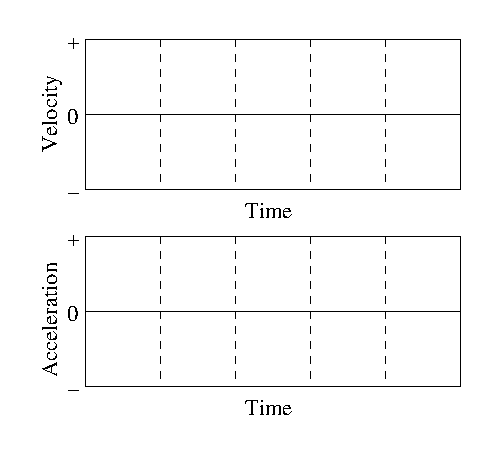
\includegraphics{slowing/slowing_fig15.eps} \par}
\vspace{0.3cm}

14. Each of the pictures below represents a car driving down a road. The motion
of the car is described. In each case, draw velocity and acceleration vectors
above the car which might represent the described motion. Also specify the sign
of the velocity and the sign of the acceleration. (The positive direction is toward the right.)

(a) The driver has stepped on the accelerator and the car is just starting to
move forward.

\vspace{0.3cm}
{\par\centering 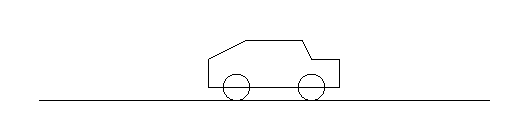
\includegraphics{slowing/slowing_fig16.eps} \par}
\vspace{0.3cm}

(b) The car is moving forward. The brakes have been applied. The car is slowing
down, but has not yet come to rest.

\vspace{0.3cm}
{\par\centering 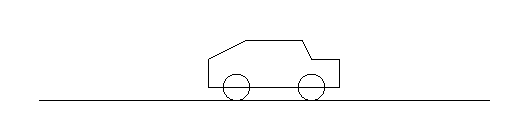
\includegraphics{slowing/slowing_fig16.eps} \par}
\vspace{0.3cm}

(c) The car is moving backward. The brakes have been applied. The car is slowing down, but has not yet come to rest.

\vspace{0.3cm}
{\par\centering 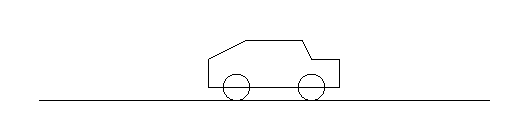
\includegraphics{slowing/slowing_fig16.eps} \par}
\vspace{0.3cm}

\newpage

The following graphs represent the motions of objects along the positive position axis. Notice that the motion of the objects is represented by position, velocity, or acceleration graphs.

Answer the following questions. You may use a graph more than once or not at
all, and there may be more correct choices than blanks. If none of the graphs
is correct, answer none.

\vspace{0.3cm}
{\par\centering 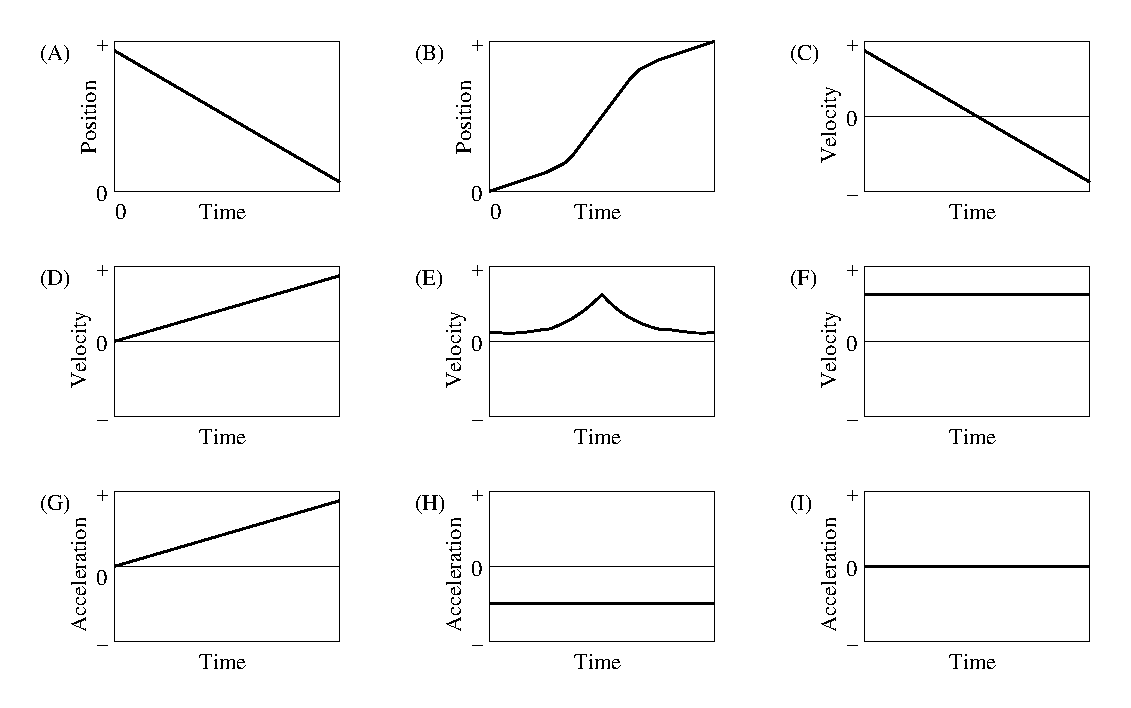
\includegraphics[trim={0.2cm 0 0.2cm 0},clip,width=\textwidth]{slowing/slowing_fig17.eps} \par}
\vspace{0.3cm}

15. Pick one graph that gives enough information to indicate that the velocity
is always negative. \rule{0.5in}{0.1pt}

Pick three graphs that represent the motion of an object whose velocity is constant.

16. \rule{0.5in}{0.1pt} 17. \rule{0.5in}{0.1pt} 18. \rule{0.5in}{0.1pt}

19. Pick one graph that definitely indicates an object has reversed direction.
\rule{0.5in}{0.1pt}

20. Pick one graph that might possibly be that of an object standing still.
\rule{0.5in}{0.1pt}

Pick 3 graphs that represent the motion of objects whose acceleration is changing.

21. \rule{0.5in}{0.1pt} 22. \rule{0.5in}{0.1pt} 23. \rule{0.5in}{0.1pt}

Pick a velocity graph and an acceleration graph that could describe the motion
of the same object during the time shown.

24. Velocity graph. \rule{0.5in}{0.1pt} 25. Acceleration graph. \rule{0.5in}{0.1pt}

